%!TEX root = ../report.tex
\chapter{Hardware Architecture}
\label{ch:hardware}
This section describes the hardware architecture of SFM. The description will be more high-level along with explanations about the hardware platform and the application interfaces between each components of the system. The rest of this chapter is organized as follows; First section, \autoref{sec:hardware-overview}, presents an overview of the hardware implemented in this system depicted in big schema. Decisions made in this system are detailed in \autoref{sec:hardware-decisions} with tables. Lastly, the hardware is described in \autoref{sec:hardware-description}.

\section{Hardware Overview}
\label{sec:hardware-overview}
The SFM hardware components can be categorized into three main components: sensing part, data storing part, and analytics part. The data flow starts from wired and wireless sensors located across the Netherlands that collect information for monitoring. UAV will also fly to gather additional information if needed. The overview of the hardware and its application interfaces are depicted in \autoref{fig:hardware-archi-schema} below.

% btw is it suppose to be the other way around? sensor monitoring -> analytics-> database ?
%\begin{figure}[hb!]
%\centering
%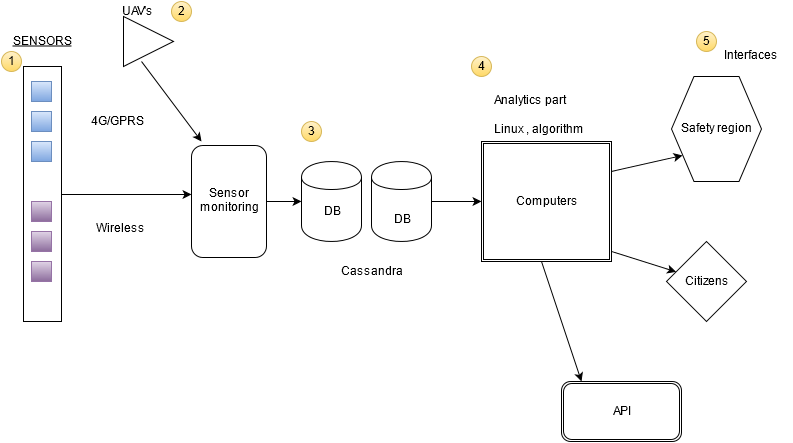
\includegraphics[scale=0.5]{images/HardwareArchitectureOverview.png}
%\caption{Schematic overview of the hardware architecture of \ProjectName{}}
%\label{fig:hardware-archi-schema}
%\end{figure}
\begin{figure}[hb!]
\centering
\includegraphics[scale=0.4]{6-hardware/images/hardwareoverview.png}
\caption{Schematic overview of the hardware architecture of \ProjectName{}}
\label{fig:hardware-archi-schema}
\end{figure}

The SFM will utilize wired and wireless sensors to monitor water ways and dikes. Wired sensors will be used for dikes monitoring and wireless sensor will be used to monitor water level. Sensors are not directly connected to the main clusters, instead, it will be connected to Arduino and then will be sent periodically using wired Internet connection through telecoms provider's line. An Arduino will be handling several sensors at once.

UAVs will also fly to check reported faulty sensors if needed. UAVs will also be used to take required pictures for further analytics or to examine some portion of the system which is hard or impossible for a personnel to access.

All incoming data will be handled by Data Collecting System in the data centers. This system is also responsible to check any incorrect data input or any faulty sensors. The next part of the hardware is the cluster for carrying out analysis. This will be a collection of servers that are coordinated using clusters. SFM will use another cluster to store important data. This cluster will run Elasticsearch database on top if it..

The last part of the hardware architecture is third party data gathering cluster. Third party data gathering cluster is responsible for collecting weather forecast and demographic information of the Netherlands. This cluster is also part of main analytics clusters.

The SFM will have several data centers to keep the system reliable running as reliability and availability is SFM's key drivers. Two of them will be inside the Netherlands and the other one will be located abroad. In this way, the system will be running correctly in case both national data centers go down.

\section{Hardware Design Decisions}
\label{sec:hardware-decisions}
This section defines decisions made regarding the hardware selection. Tables will be used to make our justification in regard to hardware selection more crystal clear.

% ng180levee
\begin{table}[h!]
\begin{tabular}{L{0.2\textwidth} L{0.6\textwidth}}
    \textbf{Name}           & \textbf{Choice of dike sensor} \\ \toprule
    \textbf{Decision}       & \textbf{HW-\textbf{\nextNrRef{hw}}}\\ \midrule
    \textbf{Status}         & \textbf{Approved} \\ \midrule
    \textbf{Problem/Issue}  & The system needs a reliable sensor system to measure condition of dikes. \\ \midrule
    \textbf{Decision}       & The system will implement GeoBeads MEMS Sensor in dikes.\\ \midrule
    \textbf{Alternatives}   & \textit{GeoBeads}\\
                            & The GeoBead is a compact sensor, which can measure the pore pressure, temperature and local tilt in dikes. A unit costs about 350 dollar\cite{ng180levee}. \\
                            & \textit{Piezometers}\\
                            & Piezometers measure the pore water pressure in the dikes. This information can be used to measure the stability of the dike. A piezometer costs about 200 dollar\cite{ng180levee}. \\
                            & \textit{Volt meters} \\
                            & Volt meters can be used to measure the streaming potential in the dike, which are an indicator of its stability\cite{selfpotential}. These sensors are approximately 50 dollars per unit. Materials in the dike can decrease the accuracy of this measurement technique. \\
                            \midrule
    \textbf{Arguments}      & \\
                            &   \begin{tabular}{l|lllllll|l}
                            &       \rot{Reliability} & \rot{Resilience} & \rot{Interoperability} & \rot{Cost} & \rot{\textbf{Score}} \\ \hline
                            %                  rel res int cost
                                    GeoBeads   & 5 & 4 & 3 & 2 & 14\\ 
                                    Piezometer & 4 & 2 & 2 & 3 & 11\\
                                    Volt meters& 1 & 5 & 2 & 5 & 13\\
                                \end{tabular} \\
    \\ \bottomrule
\end{tabular}
\caption{Decision -- Choice of Sensors}
\label{table:linux}
\end{table}


% ng180levee
\begin{table}[h!]
\begin{tabular}{L{0.2\textwidth} L{0.6\textwidth}}
    \textbf{Name}           & \textbf{Connectivity of the dike sensor} \\ \toprule
    \textbf{Decision}       & \textbf{HW-\textbf{\nextNrRef{hw}}}\\ \midrule
    \textbf{Status}         & \textbf{New} \\ \midrule
    \textbf{Problem/Issue}  & The dike sensors have to be connected to the internet in some way, so they can send their data to the central server. \\ \midrule
    \textbf{Decision}       & The sensors will be connected by a wire.\\ \midrule
    \textbf{Alternatives}   & \textit{Wired}\\
                            & A wired cable connects the dike sensor. This cable can also be used to supply the sensor with electricity. \\
                            & \textit{ZigBee}\\
                            & ZigBee is an open protocol for personal area networks. It uses little power and is therefore a good choice for devices equipped with a battery. \\
                            & \textit{ISM radio band} \\
                            & The ISM radio bands can be used for industrial, scientific and medical purposes.  \\
                            \midrule
    \textbf{Arguments}      & ZigBee is not an option, since the sensors are embedded in the soil of the dikes, and the frequency it uses, decreases too much in strength when traveling through the dike\cite{van2009draadloos}. \\
                            & Research has been done by van der Gees and Kok \cite{van2009draadloos} to determine if it is feasible to use the ISM radio band to communicate from within the dike. They concluded that, while it is possible to communicate through the dike using this band, the distance is limited and the rate of error is relatively high.
                            \\
                            & While a wire is not ideal in the sense that it will have to connect all the sensors, it seems to be the best option for the sensor in the dikes. It has the additional benefit that it can also supply the sensors with electricity.
    \\ \bottomrule
\end{tabular}
\caption{Decision -- Connectivity of the dike sensor}
\label{table:linux}
\end{table}

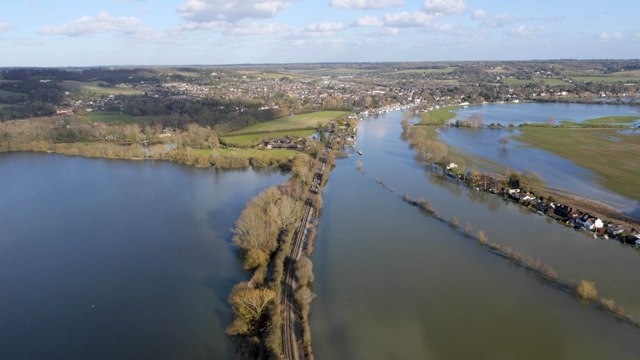
\includegraphics[scale=0.5]{6-hardware/images/uavflood.jpg}
\begin{table}[h!]
\begin{tabular}{L{0.2\textwidth} L{0.6\textwidth}}

    \textbf{Name}           & \textbf{UAVs} \\ \toprule
    \textbf{Decision}       & \textbf{DEC-2}\\ \midrule
    \textbf{Status}         & \textbf{Approved} \\ \midrule
    \textbf{Problem/Issue}  & The system uses UAV's in order to get more data during a flood and to create a map of the flooded area. \\ \midrule
    \textbf{Alternatives}   & \textit{Skyjib 8 Titanium}\\
                            &  Flight mode : GPS, computer based, Time of flight :  12-25 min  , Speed : 12m/s.\\
                            & \textit {DJI Phantom 3}\\
                            & Flight mode : GPS, comupter based, Time of flight : 15 minutes , Speed : 10 m/s .\\
                            & \textit {Skyjib Super 6 Ti-QR}\\
                            & Flight mode : GPS, comupter based, Time of flight : 10 minutes , Speed : 10 m/s . Can only support GroPro.\\ 
                            \midrule
    \textbf{Arguments}     & Getting high quality data quickly : photograph and 306 deg videos . Produce accurate and high resolution surveys .\\
                           & Cost effective. \\ 
                           & View to hard-to-reach and dangerous(where the man cannot go) areas which ensures safety because it does not require personnel to enter potentially hazardous environments. \\                          
                           & Establishment of Elevation Models to assess water flow direction and accumulation,. \\ 
                           
                               

    \\ \bottomrule
\end{tabular}
\caption{Decision -- UAVs}
\label{table:linux}
\end{table}


\begin{table}[h!]
\begin{tabular}{L{0.2\textwidth} L{0.6\textwidth}}
    \textbf{Name}           & \textbf{Analytic cluster selection} \\ \toprule
    \textbf{Decision}       & \textbf{HW-\textbf{\nextNrRef{hw}}}\\ \midrule
    \textbf{Status}         & \textbf{Approved} \\ \midrule
    \textbf{Problem/Issue}  & SFM needs a reliable computers to do the analytical processing. \\ \midrule
    \textbf{Decision}       & SFM will use clustered Dell PowerEdge R530 to act as the main analytic cluster and to provide API to the actors.\\ \midrule
    \textbf{Alternatives}   & \textit{HP ProLiant DL360 Gen9 Base}\\
                            % https://www.google.nl/shopping/product/12299869794181781707?biw=1346&bih=669&q=servers&bav=on.2,or.r_cp.&bvm=bv.104317490,d.d2s&ion=1&espv=2&tch=1&ech=1&psi=1FIQVpOAEoPlaK7Zn4AN.1443910356406.15#sgro=om
                            & This server rack has 16GB of memory and 2.4GHz of processor speed. As other server computer, this machine utilizes Intel Xeon E5 2600v3. This server is suitable for high dense computing, however the price is not so suitable for this kind of specification. It does not have LCD screen that will help technician to look the current status of the server.\\
                            & \textit{Lenovo System x3550 M4 7914}\\
                            % https://www.google.nl/shopping/product/8704926690761174474?q=servers&biw=1346&bih=669&bav=on.2,or.r_cp.&bvm=bv.104317490,d.d2s&ion=1&espv=2&tch=1&ech=1&psi=1FIQVpOAEoPlaK7Zn4AN.1443910356406.17
                            & This server rack has only 8GB of memory. However, the processor is a bit faster, it runs on 2.6GHz. As other server computer, this machine also utilizes Intel XEON E5-2600. The price is a little bit lower than the others but the memory limitation makes it not so valuable. It has LCD screen that will help technician to look the current status of the server. \\
                            & \textit{Dell PowerEdge R530} \\
                            % https://azerty.nl/0-3031-817940/dell-poweredge-r530-server-rack-uitvoering-2u-2-weg-1-x-xeon-e5-2620v3-2-4-ghz-ram-16-gb-sas-hot-swap-verwiss.html?channel_code=544&s2m_campaign=1CENT&s2m_product_id=817940
                            & This 2U server rack has 16GB of memory and 2.4GHz of processor speed. This machine utilizes Intel Xeon E5-2620V3 with 15MB of cache. This server is suitable for high dense computing. It has LCD screen that will help technician to look the current status of the server. \\
                            \midrule
    \textbf{Arguments}      & \\
                            &   \begin{tabular}{l|llllll|l}
                            &       \rot{Reliability} & \rot{Performance}& \rot{Interoperability} & \rot{Security} & \rot{Scalability} & \rot{Cost} & \rot{\textbf{Score}} \\ \hline
                            %                                       rel perf int sec sca cost
                                    Dell PowerEdge R530             & 5 & 5 & 4 & 4 & 4 & 5 & 27 \\ 
                                    Lenovo System x3550 M4 7914     & 4 & 4 & 4 & 3 & 4 & 4 & 23 \\
                                    HP ProLiant DL360 Gen9 Base     & 5 & 5 & 4 & 3 & 4 & 3 & 24 \\
                                \end{tabular} \\
    \\ \bottomrule
\end{tabular}
\caption{Decision -- Analytic cluster selection}
\label{table:server-selection}
\end{table}

\begin{table}[h!]
\begin{tabular}{L{0.2\textwidth} L{0.6\textwidth}}
    \textbf{Name}           & \textbf{Database cluster selection} \\ \toprule
    \textbf{Decision}       & \textbf{HW-\textbf{\nextNrRef{hw}}}\\ \midrule
    \textbf{Status}         & \textbf{Approved} \\ \midrule
    \textbf{Problem/Issue}  & The system needs reliable computers to store the data. \\ \midrule
    \textbf{Decision}       & SFM will utilize Synology RackStation RS814RP to store the data.\\ \midrule
    \textbf{Alternatives}   & \textit{Synology RackStation RS814RP}\\
                            % https://www.google.nl/shopping/product/9793555443596138172?biw=1346&bih=669&q=storage+servers&bav=on.2,or.r_cp.&bvm=bv.104317490,d.d2s&ion=1&espv=2&tch=1&ech=1&psi=1FIQVpOAEoPlaK7Zn4AN.1443910356406.23&prds=paur:ClkAsKraX8aViW9QBHq_YeLbadvaW6lnMVQDuwzotG6gRVknHILZ_EDzrO8nQNS6N477UjRspRo17BmUoyZnQjMDnOrhflRLM5VXFQCOPDxn9wCZnGJxrWXfWxIZAFPVH73DWMclCanKIzQ68mJVd6ADLpvTfg&sa=X&ved=0CMkDEM1KMBJqFQoTCLid3qaqp8gCFYrZGgodX70Kow
                            & This storage machine has the fastest connection among the others. This machine will run at SATA with 6 Gbps connection.\\
                            & \textit{70BJ NAS-server}\\
                            % https://www.google.nl/shopping/product/15463250681911940369?q=storage+servers&biw=1346&bih=669&bav=on.2,or.r_cp.&bvm=bv.104317490,d.d2s&ion=1&espv=2&tch=1&ech=1&psi=1FIQVpOAEoPlaK7Zn4AN.1443910356406.25&prds=paur:ClkAsKraXy1_BVqi5aD5CGi7OmupTi3OwyL-j7nW7Ss2Qwo-W_81sjaidQU8J0Q3uu7RrSCCth3c9YuMEMNA3zO6TM9tfutSn6ksUeo1EGFdUDKUIlB4gt8wBBIZAFPVH70byN_Dqe5qhSCABb7sxVXYXAvfaw&sa=X&ved=0CIEDEM1KMAo4FGoVChMIpJb_tKqnyAIVQUwaCh0d6wGT
                            & This machine form factor is 1U which is suitable for saving space. However, the connection speed is limited to 3 Gbps.\\
                            & \textit{Thecus N8810U-G NAS-server} \\
                            % https://www.google.nl/shopping/product/464537487289413504?q=storage+servers&biw=1346&bih=669&bav=on.2,or.r_cp.&bvm=bv.104317490,d.d2s&ion=1&espv=2&tch=1&ech=1&psi=1FIQVpOAEoPlaK7Zn4AN.1443910356406.25&prds=paur:ClkAsKraXylXtQJRG2pDp_XW-OBbRHsXe6nrmcB3olgeJQi1FhG4T8bXQABWVbkevi6hzBMwfTk7qioWd88Cq3GWIt3hQlEi5oJEmR7vZvXtvtEinYYlhn3_bBIZAFPVH71qflxmS1BuYghV4B5tpcohhFU7vQ&sa=X&ved=0CNQCEM1KMAU4FGoVChMIpJb_tKqnyAIVQUwaCh0d6wGT
                            & This machine also runs in 3Gbps connection. However, the form factor is 2U which makes this machine takes more space in the rack.\\
                            \midrule
    \textbf{Arguments}      & \\
                            &   \begin{tabular}{l|llllll|l}
                            &       \rot{Reliability} & \rot{Performance}& \rot{Interoperability} & \rot{Security} & \rot{Scalability} & \rot{Cost} & \rot{\textbf{Score}} \\ \hline
                            %                                       rel perf int sec sca cost
                            Synology RackStation RS814RP    & 5 & 4 & 4 & 4 & 4 & 4 & 25 \\ 
                            70BJ NAS-server                 & 4 & 3 & 4 & 4 & 4 & 3 & 22 \\
                            Thecus N8810U-G NAS-server      & 4 & 3 & 4 & 4 & 4 & 3 & 22 \\
                                \end{tabular} \\
    \\ \bottomrule
\end{tabular}
\caption{Decision -- Choice of storage machine.}
\label{table:database-selection}
\end{table}

\begin{table}[h!]
\begin{tabular}{L{0.2\textwidth} L{0.6\textwidth}}
    \textbf{Name}           & \textbf{High Performance Switch selection} \\ \toprule
    \textbf{Decision}       & \textbf{HW-\textbf{\nextNrRef{hw}}}\\ \midrule
    \textbf{Status}         & \textbf{Approved} \\ \midrule
    \textbf{Problem/Issue}  & SFM cluster needs a powerful high performance switch to connect each cluster. \\ \midrule
    \textbf{Decision}       & SFM will use Cisco Catalyst 2960S-24TS-L Switch.\\ \midrule
    \textbf{Alternatives}   & \textit{Linksys LGS552P Switch}\\
                            % https://www.google.nl/shopping/product/15955701749855379542?biw=1346&bih=669&q=network+switch&sqi=2&bav=on.2,or.r_cp.&bvm=bv.104317490,d.d2s&ion=1&espv=2&tch=1&ech=1&psi=1FIQVpOAEoPlaK7Zn4AN.1443910356406.33&prds=paur:ClkAsKraX5ryPFpohZJ3cHRR5Y04pVrqqvR-5nXru2N7X2-97H3V7DAZtCjwWh2BPthulxNJ2ahSWe7PR9qBPpG4AcckL_q3UHXeyd1fqIcsRCo9aEhM_4ihYhIZAFPVH7186CU9loBEx5Tx9iwfjvLu2xB6eg&sa=X&ved=0CM4CEM1KMAJqFQoTCJaXr-ahqMgCFUh-Ggodym4G5w
                            & This switch has 52 ports available for connection, which is very good for scalability. However the performance is not as good as Cisco catalyst switch series.\\
                            & \textit{HP 1820-48G Switch}\\
                            % https://www.google.nl/shopping/product/7539423950361123669?biw=1346&bih=669&q=network+switch&sqi=2&bav=on.2,or.r_cp.&bvm=bv.104317490,d.d2s&ion=1&espv=2&tch=1&ech=1&psi=1FIQVpOAEoPlaK7Zn4AN.1443910356406.33&prds=paur:ClkAsKraX2rp4gF8ATRwWJuY5iaZuchaa1sdhIz6lvepgxugqRb5mZxy8yAXts_70QyVg33fwd3C8WiFm3ThxDkZDi6gz2-ogcVLZ1Frs8QHH9IhEd-rj9s-CBIZAFPVH71WuYA_yyIRCl_FpDi93AJr9DX5QQ&sa=X&ved=0CNgCEM1KMANqFQoTCJaXr-ahqMgCFUh-Ggodym4G5w
                            & This switch has lesser available ports than Linksys switch. It has 48 ports available. This switch is not very configurable which makes this not so suitable for high performance switching. \\
                            & \textit{Cisco Catalyst 2960S-24TS-L Switch} \\
                            % https://www.google.nl/shopping/product/3278668597556943908?biw=1346&bih=669&q=network+switch&sqi=2&bav=on.2,or.r_cp.&bvm=bv.104317490,d.d2s&ion=1&espv=2&tch=1&ech=1&psi=1FIQVpOAEoPlaK7Zn4AN.1443910356406.33&prds=paur:ClkAsKraXw_7YyEqvAKzRJjfEM3yN-4kzC4NaE-smcis8WFMegcToXlCuBmXRPb647qqqZU34GfFxp8EYHh7FC1AVCwaCRNTWcvFYI4Ppe8B8xT_2AMPJ7r3XBIZAFPVH72nlGbb8LwIOpZWGX8ZHfTvUUmDSw&sa=X&ved=0CPUCEM1KMAZqFQoTCJaXr-ahqMgCFUh-Ggodym4G5w
                            & This switch has the lowest number of port available, 24 ports. However, Cisco Catalyst is very configurable and has a very good security. \\
                            \midrule
    \textbf{Arguments}      & \\
                            &   \begin{tabular}{l|llllll|l}
                            &       \rot{Reliability} & \rot{Performance}& \rot{Interoperability} & \rot{Security} & \rot{Scalability} & \rot{Cost} & \rot{\textbf{Score}} \\ \hline
                            %                                   rel perf int sec sca cost
                            Cisco Catalyst 2960S-24TS-L Switch  & 5 & 5 & 4 & 5 & 3 & 4 & 26 \\ 
                            Linksys LGS552P Switch              & 4 & 4 & 4 & 3 & 4 & 5 & 24 \\
                            HP 1820-48G Switch                  & 3 & 4 & 4 & 3 & 4 & 5 & 23 \\
                                \end{tabular} \\
    \\ \bottomrule
\end{tabular}
\caption{Decision -- Choice of high performance switch}
\label{table:switch-selection}
\end{table}


\clearpage
\section{Hardware Description}
\label{sec:hardware-description}
% Mention the difference between previous chapter
This section gives an outline of the hardware implemented in this system. This section also elaborates on hardware decisions.

\subsection{Sensor Components}
\label{subsec:sensing-components}
Roughly 17.000 kilometers of dikes protect the Netherlands against flooding\cite{DMC}. Of this, about 3.500 kilometers are primary dikes\cite{waterwijzer}. These are dikes protecting against the water of the sea, the big rivers (Rijn, Maas, IJssel), the IJsselmeer and the Markermeer. 

The hardware architecture of the system is composed of two sensor components. The first sensor component are sensors installed in the dikes to measure and detect potential instability of the dikes.
The second sensing component consists of water level sensors, which are spread along water ways in the country, to measure the water level. 

\label{dikesensors}
\subsubsection*{Dike sensors}
To measure the stability of the dikes, the GeoBeads dike monitoring sensor will be installed in the dikes. When these sensors are placed in the dike with a spacing of 3 meters, they will provide optimal measurements\cite{ng180levee}. The GeoBead will measure the water pressure, temperature, inclination and acceleration.

A GeoBead sensor consists of several modules, loosely connected by cable, which form a chain of sensors. The GeoBeads will be installed in a pre-drilled vertical hole, or where this is not possible, horizontally. Three sensors are installed per cross-section and a cross-section is installed every 100 m. 

The GeoBeads cannot send their data directly to the central server. Therefore, at each cross-section, there will be a module (consisting of an Arduino in a water-proof casing), which is responsible for processing and sending the data to the central server using cable internet.

The GeoBeads are connected by communication cable, and a cable for the power supply. 

\subsubsection*{Water level sensors}
The water level sensors are placed next to the dikes and in the water ways. The water level sensors are placed more scattered than the dike sensors. The water level sensors are also connected to an Arduino for processing and sending the data. The water level sensor are also connected to a solar cell and a battery for power supply.

The water level sensors are accommodated with a connectivity chip, which allows it to use the mobile broadband to connect to the central server.
% TODO: decide on exact water level sensor

\subsection{UAV's }
Goals : Flood monitoring and flood damage assessment
UAVs provide a way for us to assess more accurately the impacts of climate change and flooding,
The system will use UAV's in order to get more accurate data , and high resolution photographs and videos in order to map the flooded area.
 
High resolution elevation models for accurate predictions of flood extent thresholds and flow accumulation analysis. Elevation models can also be used to accurately measure changes to the physical land, such as landslides.

GPS, which allows te system to input coordinates in advance to map out the perfect flight plan.
% Operator , commander to pilot 
The UAV's won't fly everytime , they will be released during the risky periods of flood.

%The UAV will be equiped with camera ....

% Server specs
% - Server
% - Networking device
% - UPS

\clearpage
\subsection{Database Cluster and Data Collection}
\label{subsec:database-data}
In the previous chapter, SFM will use Cassandra database as the database platform. However, Cassandra requires computers to run its environment. SFM will use clusters of computer to manage database system and to store our data. The cluster will also be accessible by the main analytics part as the data will come and go through the main analytics part. The logical schematic of the database cluster is depicted in \autoref{fig:database-cluster}

\begin{figure}[hb!]
\centering
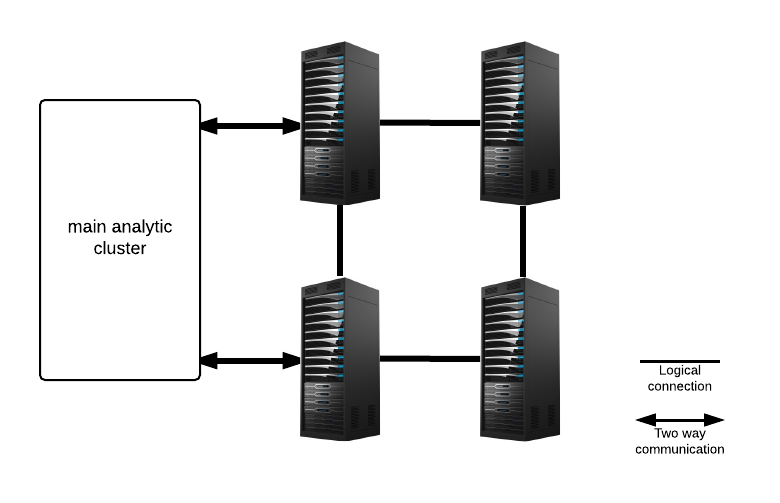
\includegraphics[width=0.7\textwidth]{6-hardware/images/db-cluster.png}
\caption{Logical schematic of database cluster of SFM}
\label{fig:database-cluster}
\end{figure}

As can be seen in \autoref{fig:database-cluster}, SFM will use four database racks to have redundancy in the system. The database cluster By using this form of architecture, SFM will be more reliable and fault tolerant. There will also be two physical connection to the main analytic cluster to make this system more fault tolerant in terms of connection. SFM database cluster will use the same server, Dell PowerEdge R530, for controlling the SATA storage machine.

% Clustering, in the context of databases, refers to the ability of several servers or instances to connect to a single database. An instance is the collection of memory and processes that interacts with a database, which is the set of physical files that actually store data.

% Clustering offers two major advantages, especially in high-volume database environments:

% Fault tolerance: Because there is more than one server or instance for users to connect to, clustering offers an alternative, in the event of individual server failure.
% Load balancing: The clustering feature is usually set up to allow users to be automatically allocated to the server with the least load.

% Adds some picture here

\subsection{Analytics Components}
\label{subsec:analytics}
Analytics component will be the main brain of SFM. The intelligent algorithm will run on this machine. This components are also responsible for checking faulty sensors by analyzing incoming sensor data. Thus, there is a big dependency to this components. To increase availability and reliability, SFM will have six server racks to do the processing as depicted in \autoref{fig:analytic-cluster}.

\begin{figure}[hb!]
\centering
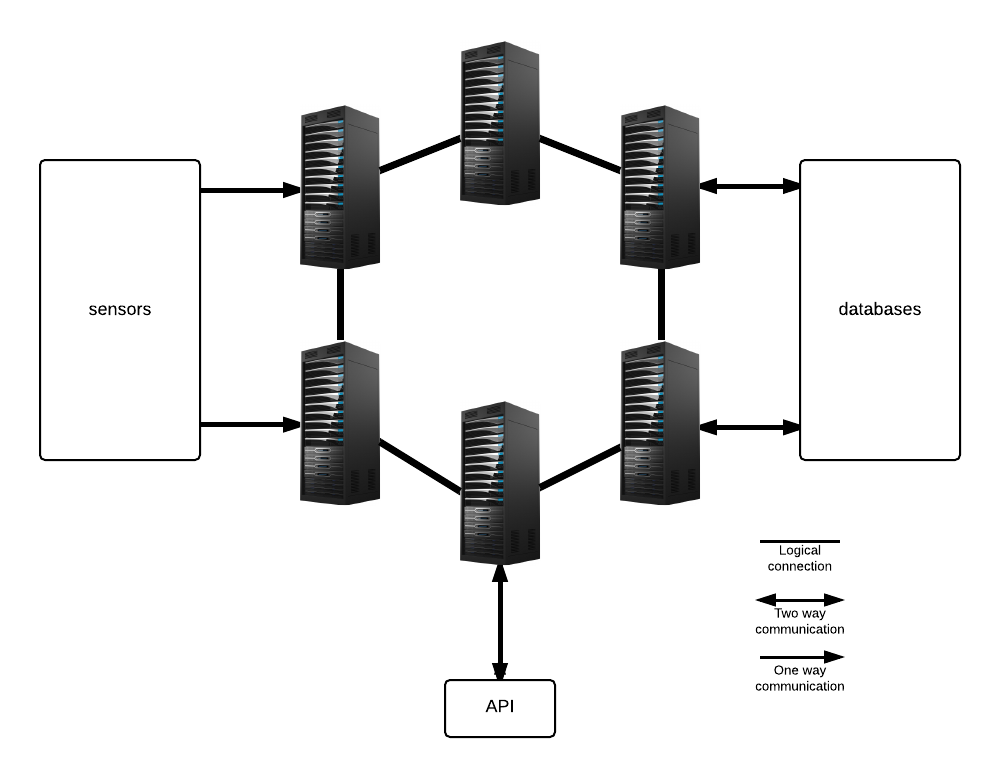
\includegraphics[width=0.7\textwidth]{6-hardware/images/analytic-cluster.png}
\caption{Logical schematic of analytic cluster of SFM}
\label{fig:analytic-cluster}
\end{figure}

The analytics components will also be the hub for the main connection of SFM. Thus, this system also need a high performance switch to accomplish this purpose. As have been mentioned before, this system will use Cisco Catalyst 2960S-24TS-L Switch.

The analytics components will use Dell PowerEdge R530 as server and it will be mounted on a server rack. The detailed hardware specifications of Dell PowerEdge R530 is listed in \autoref{table:server-specs}.

\begin{table}[!htbp]
    \centering
    \begin{tabular}{L{\tw{0.2}} L{\tw{0.4}}}
    \toprule
    \multicolumn{2}{c}{Dell PowerEdge R530 Specification} \\ \midrule
    \textbf{Item Description} & Dell PowerEdge R530 - E5-2620V3 Xeon 2.4 GHz - 16 GB - 1 TB \\
    \textbf{Type} & Server - rack-mountable \\
    \textbf{Height (Rack Units)} & 2U \\
    \textbf{Processor} & 1 x Intel Xeon E5-2620V3 / 2.4 GHz (3.2 GHz) (6-core) \\
    \textbf{Processor Main Features} & Intel Turbo Boost Technology 2 \\
    \textbf{Cache Memory} & 15 MB \\
    \textbf{Cache per processor} & 15 MB \\
    \textbf{RAM} & 16 GB (installed) / 384 GB (max.) - DDR4 SDRAM - 2133 MHz \\
    \textbf{Storage Controller} & RAID (SATA 6Gb / s) (Dell PERC H330) \\
    \textbf{Optical Storage} & DVD burner \\
    \textbf{Graphics Controller} & Matrox G200 \\
    \textbf{Video Memory} & 16 MB \\
    \textbf{Network} & GigE \\
    \textbf{Dimensions} &  (WxDxH)48.24 cm x 64.6 cm x 8.68 cm \\
    \textbf{Weight} & 2.14 kg \\
    \bottomrule
    \end{tabular}
\caption{Hardware specification of Dell PowerEdge R530}
\label{table:server-specs}
\end{table}


% Server specs
% - Server
% - Networking device
% - UPS